\documentclass[tikz,border=5pt]{standalone}
\usepackage[utf8]{inputenc}
\usepackage[T1]{fontenc}
\usepackage{lmodern,amsmath,amssymb}
\usepackage[american]{circuitikz}
\usepackage{pgfplots}
\pgfplotsset{compat=1.18}
\usetikzlibrary{circuits.logic.US,positioning,calc,arrows.meta,patterns,shapes.geometric}
\definecolor{Primary}{HTML}{1F77B4}
\begin{document}
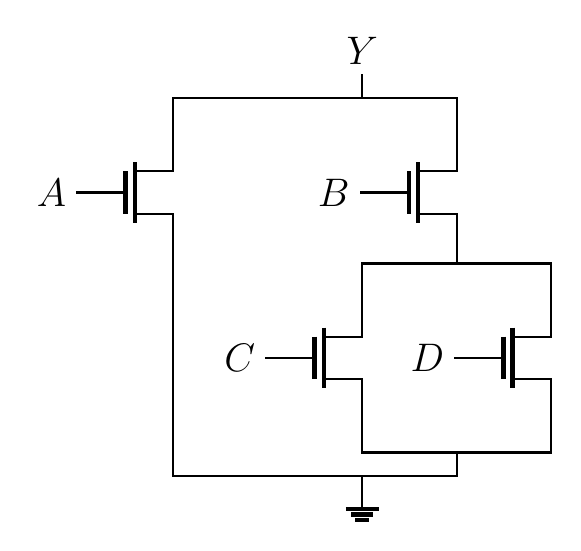
\begin{tikzpicture}[thick,font=\Large]\draw(0,0)--(-2.3999999999999995,0)--(-2.3999999999999995,-0.3);\node[nmos](m21)at(-2.3999999999999995,-1.2){};\draw(-2.3999999999999995,-0.3)--(m21.D)(m21.S)--(-2.3999999999999995,-2.1);\draw(m21.G)--++(-.25,0)node[left]{$A$};\draw(-2.3999999999999995,-2.1)--(-2.3999999999999995,-4.8)--(0,-4.8);\draw(0,0)--(1.2000000000000002,0)--(1.2000000000000002,-0.3);\node[nmos](m22)at(1.2000000000000002,-1.2){};\draw(1.2000000000000002,-0.3)--(m22.D)(m22.S)--(1.2000000000000002,-2.1);\draw(m22.G)--++(-.25,0)node[left]{$B$};\draw(1.2000000000000002,-2.1)--(2.220446049250313e-16,-2.1)--(2.220446049250313e-16,-2.4);\node[nmos](m23)at(2.220446049250313e-16,-3.3){};\draw(2.220446049250313e-16,-2.4)--(m23.D)(m23.S)--(2.220446049250313e-16,-4.2);\draw(m23.G)--++(-.25,0)node[left]{$C$};\draw(2.220446049250313e-16,-4.2)--(2.220446049250313e-16,-4.5)--(1.2000000000000002,-4.5);\draw(1.2000000000000002,-2.1)--(2.4000000000000004,-2.1)--(2.4000000000000004,-2.4);\node[nmos](m24)at(2.4000000000000004,-3.3){};\draw(2.4000000000000004,-2.4)--(m24.D)(m24.S)--(2.4000000000000004,-4.2);\draw(m24.G)--++(-.25,0)node[left]{$D$};\draw(2.4000000000000004,-4.2)--(2.4000000000000004,-4.5)--(1.2000000000000002,-4.5);\draw(1.2000000000000002,-4.5)--(1.2000000000000002,-4.8)--(0,-4.8);\draw(0,0)--++(0,.3)node[above]{$Y$};\draw(0,-4.8)node[ground]{};\end{tikzpicture}
\end{document}
